\documentclass{beamer}
\usepackage[numbers]{natbib}

\setbeamerfont{caption}{series=\normalfont,size=\fontsize{8}{15}} 

\usetheme{Madrid}

\title{Analysing and Predicting Xbox Game Sales using
Machine Learning}
\author{Josh Cox}
\institute{University Of Exeter}
\date{2023}

\begin{document}

\frame{\titlepage}

% -------------- Research Question --------------
\begin{frame}
\frametitle{Research Question}

\begin{itemize}
\setlength\itemsep{1em}
    \item Can we use machine learning to predict the sales of an Xbox game in different parts of the world?
    \item This is useful for upcoming games:
    \medskip
    \begin{itemize}
    \setlength\itemsep{1em}
        \item Change the level of marketing in different areas
        \item Different pricing of the game depending on the area
        \item Some games might only release in certain areas
    \end{itemize}
\end{itemize}

\end{frame}

% -------------- Dataset --------------

\begin{frame}{Dataset}

\begin{itemize}
    \item 613 Xbox games from 2013 to 2020 \cite{noauthor_video_nodate}
    \item Columns we will be using:
    \begin{itemize}
        \item Genre - The genre of the game
        \item Publisher - Publisher that released the game
        \item North America - Sales in North America
        \item Europe - Sales in Europe
        \item Japan - Sales in Japan
        \item Rest of World - Sales in other areas
    \end{itemize}
\end{itemize}

\begin{figure}
\centering
    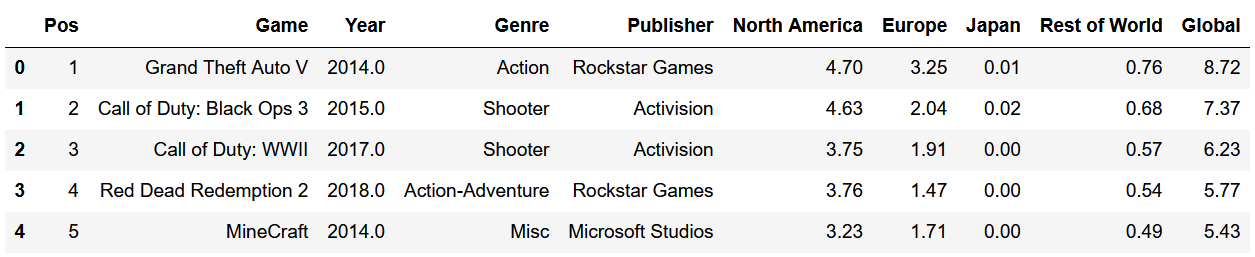
\includegraphics[width=1\textwidth]{img/games_dataset.png}
    \vspace{-8mm}
    \caption{Xbox game dataset}
\end{figure}

\end{frame}

% -------------- Preprocessing --------------

\begin{frame}{Preprocessing}


\begin{itemize}
\item Removed unwanted columns
\begin{itemize}
    \item Game name, Year of Release, Global Sales, Position
\end{itemize}
\vspace{3mm}
\item Formatted data
\begin{itemize}
    \item Changed column names and converted to lowercase
    \item Encoded categorical data
    \item Scaled data
\end{itemize}
\end{itemize}

\vspace{3mm}

\begin{figure}
\centering
    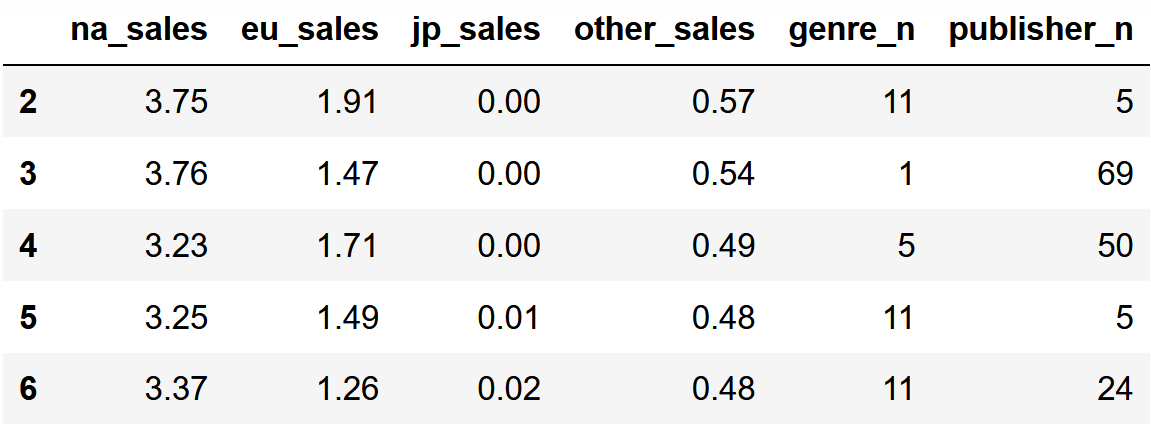
\includegraphics[width=0.7\textwidth]{img/formatted_data.png}
        \vspace{-2mm}
    \caption{Preprocessed dataset}
\end{figure}


\end{frame}

% -------------- Outliers --------------

\begin{frame}{Check for Outliers}

\begin{itemize}
    \item Checked for outliers
    \begin{itemize}
        \item Using Interquartile Range (IQR) isn't applicable
        \item Used visualisation of data
    \end{itemize}
\end{itemize}

\begin{center}  
    \begin{figure}
    \centering
        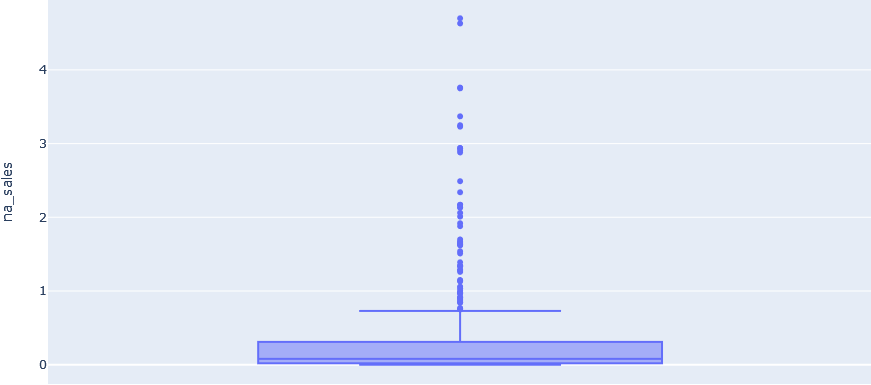
\includegraphics[width=0.9\textwidth]{img/boxplot.png}
            \vspace{-2mm}
        \caption{Box plot of data}
    \end{figure}
\end{center}

\end{frame}

% -------------- Approach --------------

\begin{frame}{Approach}

\begin{itemize}
    \item Train regression models to predict sales in each area based on:
    \begin{itemize}
        \item Genre of the game
        \item Publisher of the game
    \end{itemize}

    \vspace{3mm}

    \item Cluster the data into groups based on sales in each area
    \begin{itemize}
        \item For example one group of games did better in Europe than North America
    \end{itemize}

    \vspace{3mm}

    \item Train a classifier to organise data points into created clusters
\end{itemize}

\end{frame}

% -------------- Regression --------------

\begin{frame}{Regression}

\begin{itemize}
    \item Trained two regressors:
    \begin{itemize}
        \item Random Forest (RF)
        \item Gradient Boosting (GB)
    \end{itemize}
    
    \vspace{3mm}
    
    \item Results:
    \begin{itemize}
        \item GB outperformed RF for Europe
        \item RF outperformed GB for North America and Other
    \end{itemize}

\vspace{3mm}

\item Decide to drop Japan as not enough data points
\end{itemize}

\begin{table}[]
\begin{tabular}{c|ccl|ccl|}
\cline{2-7}
                                    & \multicolumn{3}{c|}{Random Forest}                            & \multicolumn{3}{c|}{Gradient Boosting}                        \\ \cline{2-7} 
\multicolumn{1}{l|}{}               & \multicolumn{1}{l|}{$R^2$ Score} & \multicolumn{2}{l|}{MSE}   & \multicolumn{1}{l|}{$R^2$ Score} & \multicolumn{2}{l|}{MSE}   \\ \hline
\multicolumn{1}{|c|}{North America} & \multicolumn{1}{c|}{0.495}       & \multicolumn{2}{c|}{0.226} & \multicolumn{1}{c|}{0.479}       & \multicolumn{2}{c|}{0.233} \\ \hline
\multicolumn{1}{|c|}{Europe}        & \multicolumn{1}{c|}{0.339}       & \multicolumn{2}{c|}{0.092} & \multicolumn{1}{c|}{0.343}       & \multicolumn{2}{c|}{0.091} \\ \hline
\multicolumn{1}{|c|}{Japan}         & \multicolumn{1}{c|}{-0.110}      & \multicolumn{2}{c|}{3.141} & \multicolumn{1}{c|}{-0.161}      & \multicolumn{2}{c|}{3.284} \\ \hline
\multicolumn{1}{|c|}{Other}         & \multicolumn{1}{c|}{0.476}       & \multicolumn{2}{c|}{0.005} & \multicolumn{1}{c|}{0.461}       & \multicolumn{2}{c|}{0.005} \\ \hline
\end{tabular}
\caption{Results for RF and GB Regressors}
\end{table}

\end{frame}

% -------------- Clustering --------------

\begin{frame}{Clustering}

\begin{itemize}
    \item Tested 3 clustering algorithms:
    \begin{itemize}
        \item K-Means
        \item Density-based spatial clustering of applications with noise (DBSCAN)
        \item Gaussian Mixture Model (GMM)
    \end{itemize}
\end{itemize}

\begin{columns}
    \begin{column}{0.5\textwidth}

        \begin{figure}
        \centering
            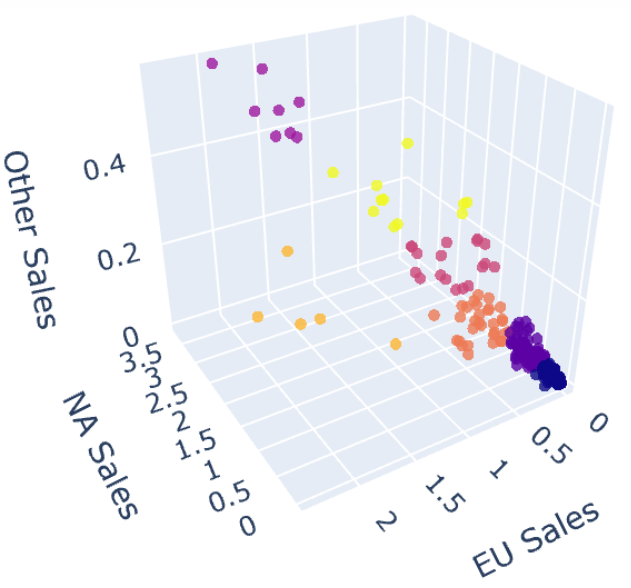
\includegraphics[width=0.7\textwidth]{img/gmm_scatter.png}
                \vspace{-2mm}
            \caption{GMM Clusters}
        \end{figure}

    \end{column}

    \begin{column}{0.5\textwidth}
        \begin{itemize}
        \item Used elbow plot and average silhouette scores to find K = 7
        \vspace{3mm}
            \item Silhouette Scores:
            \begin{itemize}
                \item K-Means: 0.961
                \item DBSCAN: 0.937
                \item GMM: 0.961
            \end{itemize}
        \end{itemize}
    \end{column}
\end{columns}



\end{frame}


\begin{frame}{Dimensionality Reduction}

 \begin{figure}
    \centering
        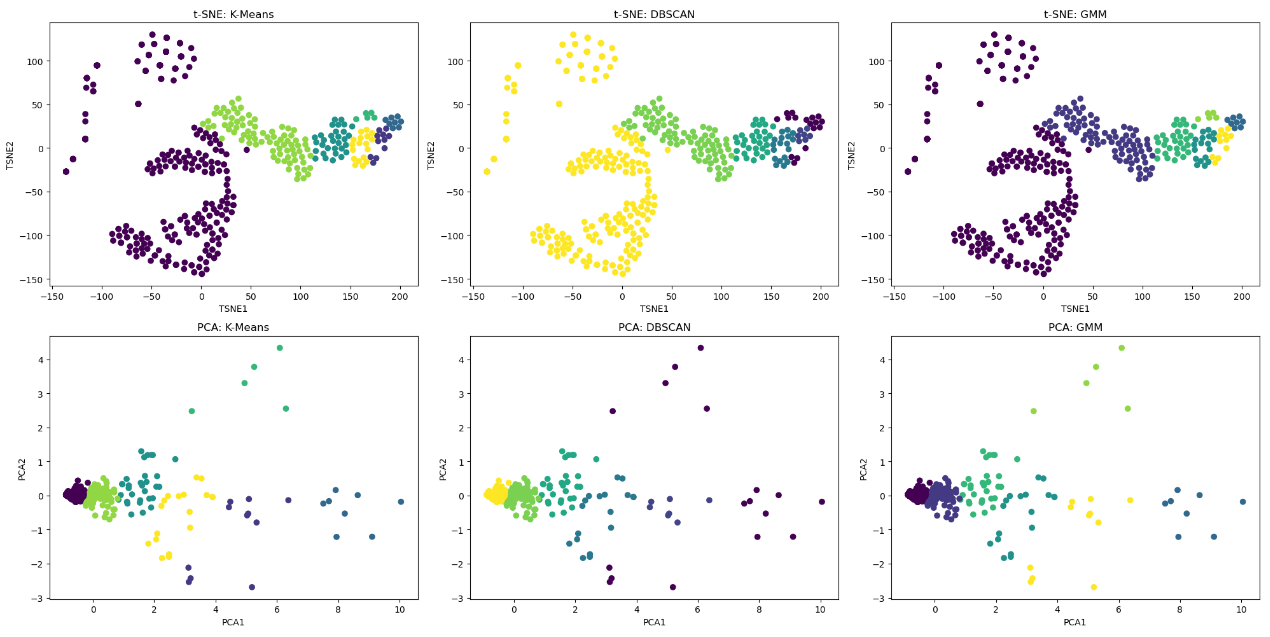
\includegraphics[width=1\textwidth]{img/dimensionality_reduction.png}
            \vspace{-6mm}
        \caption{t-SNE and PCA Scatter Plots}
\end{figure}

\end{frame}

% -------------- Classification --------------

\begin{frame}{Classification}

\begin{columns}
    \begin{column}{0.4\textwidth}
        \begin{itemize}
            \item Tested RF and GB
            \vspace{3mm}
            \item F1 Score:
            \begin{itemize}
                \item RF: 0.973
                \item GB: 0.957
            \end{itemize}
            \vspace{3mm}
            \item Mean Squared Error:
            \begin{itemize}
                \item RF: 0.119
                \item GB: 0.205
            \end{itemize}
            \vspace{3mm}
            \item Skewed results due to number of 0 values, but still accurate
        \end{itemize}
    \end{column}
    
    \begin{column}{0.7\textwidth}
         \begin{figure}
            \centering
            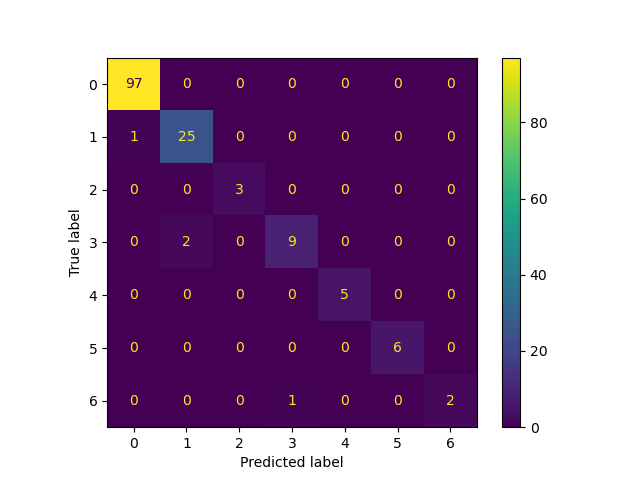
\includegraphics[width=1\textwidth]{img/confusion_matrix.png}
                \vspace{-8mm}
            \caption{RF Classifier Confusion  Matrix}
        \end{figure}

    \end{column}
\end{columns}

\end{frame}

% -------------- Conclusion --------------

\begin{frame}{Conclusion}

\begin{itemize}
    \item Predictor
    \begin{itemize}
        \item Accuracy was lacking in regressors
        \item Likely due to only using genre and publisher
    \end{itemize}
    \vspace{3mm}
    \item Clustering
    \begin{itemize}
        \item Resulted in accurate groupings
        \item Useful for organising and visualising sales of games
    \end{itemize}
    \vspace{3mm}
    \item Classifier
    \begin{itemize}
        \item Skewed due to data
        \item Provided accurate classifying of data
        \item Useful for visualising sales of a game
    \end{itemize}
\end{itemize}

\end{frame}

% -------------- Improvements --------------

\begin{frame}{Further Improvements}

\begin{itemize}
    \item Using a more complex machine learning model
    \begin{itemize}
        \item For example tuning a Neural Network
        \item Testing different architectures (number of hidden layers etc)
    \end{itemize}
    \vspace{3mm}
    \item Using more complex features
    \begin{itemize}
        \item Genre and publisher don't define a game's sales 
        \item Considering factors such as graphics, sounds, online capability etc
    \end{itemize}
\end{itemize}

\end{frame}

% -------------- References --------------

\begin{frame}{References}

\bibliographystyle{IEEEtran}
\bibliography{IEEEabrv, main}
    
\end{frame}


\end{document}